% Options for packages loaded elsewhere
\PassOptionsToPackage{unicode}{hyperref}
\PassOptionsToPackage{hyphens}{url}
%
\documentclass[
]{book}
\usepackage{lmodern}
\usepackage{amssymb,amsmath}
\usepackage{ifxetex,ifluatex}
\ifnum 0\ifxetex 1\fi\ifluatex 1\fi=0 % if pdftex
  \usepackage[T1]{fontenc}
  \usepackage[utf8]{inputenc}
  \usepackage{textcomp} % provide euro and other symbols
\else % if luatex or xetex
  \usepackage{unicode-math}
  \defaultfontfeatures{Scale=MatchLowercase}
  \defaultfontfeatures[\rmfamily]{Ligatures=TeX,Scale=1}
\fi
% Use upquote if available, for straight quotes in verbatim environments
\IfFileExists{upquote.sty}{\usepackage{upquote}}{}
\IfFileExists{microtype.sty}{% use microtype if available
  \usepackage[]{microtype}
  \UseMicrotypeSet[protrusion]{basicmath} % disable protrusion for tt fonts
}{}
\makeatletter
\@ifundefined{KOMAClassName}{% if non-KOMA class
  \IfFileExists{parskip.sty}{%
    \usepackage{parskip}
  }{% else
    \setlength{\parindent}{0pt}
    \setlength{\parskip}{6pt plus 2pt minus 1pt}}
}{% if KOMA class
  \KOMAoptions{parskip=half}}
\makeatother
\usepackage{xcolor}
\IfFileExists{xurl.sty}{\usepackage{xurl}}{} % add URL line breaks if available
\IfFileExists{bookmark.sty}{\usepackage{bookmark}}{\usepackage{hyperref}}
\hypersetup{
  pdftitle={The Examples Book},
  hidelinks,
  pdfcreator={LaTeX via pandoc}}
\urlstyle{same} % disable monospaced font for URLs
\usepackage{longtable,booktabs}
% Correct order of tables after \paragraph or \subparagraph
\usepackage{etoolbox}
\makeatletter
\patchcmd\longtable{\par}{\if@noskipsec\mbox{}\fi\par}{}{}
\makeatother
% Allow footnotes in longtable head/foot
\IfFileExists{footnotehyper.sty}{\usepackage{footnotehyper}}{\usepackage{footnote}}
\makesavenoteenv{longtable}
\usepackage{graphicx}
\makeatletter
\def\maxwidth{\ifdim\Gin@nat@width>\linewidth\linewidth\else\Gin@nat@width\fi}
\def\maxheight{\ifdim\Gin@nat@height>\textheight\textheight\else\Gin@nat@height\fi}
\makeatother
% Scale images if necessary, so that they will not overflow the page
% margins by default, and it is still possible to overwrite the defaults
% using explicit options in \includegraphics[width, height, ...]{}
\setkeys{Gin}{width=\maxwidth,height=\maxheight,keepaspectratio}
% Set default figure placement to htbp
\makeatletter
\def\fps@figure{htbp}
\makeatother
\setlength{\emergencystretch}{3em} % prevent overfull lines
\providecommand{\tightlist}{%
  \setlength{\itemsep}{0pt}\setlength{\parskip}{0pt}}
\setcounter{secnumdepth}{-\maxdimen} % remove section numbering

\title{The Examples Book}
\author{}
\date{\vspace{-2.5em}}

\begin{document}
\maketitle

{
\setcounter{tocdepth}{1}
\tableofcontents
}
\hypertarget{introduction}{%
\chapter{Introduction}\label{introduction}}

This book contains a collection of examples that students can use to reinforce topics learned in The Data Mine seminar. It is an excellent resource for students to learn what they need to know in order to solve The Data Mine projects.

\hypertarget{how-to-contribute}{%
\section{How to contribute}\label{how-to-contribute}}

Contributing to this book is simple:

\begin{enumerate}
\def\labelenumi{\arabic{enumi}.}
\item
  Navigate to the page or section that needs to be edited
\item
  Click on the ``Edit'' button towards the upper left side of the page:
  
\includegraphics{images/edit_button.png}
\item
  You'll be presented with the respective RMarkdown file. Make your modifications.
\item
  In the ``Commit changes'' box, select the radio button that says \emph{Create a \textbf{new branch} for this commit and start a pull request.} Give your pull request a title and a detailed description. Name the new branch, and click on ``Propose file change''.
\item
  You've successfully submitted a pull request. Our team will review and merge the request shortly thereafter.
\end{enumerate}

\hypertarget{scholar}{%
\chapter{Scholar}\label{scholar}}

\hypertarget{connecting-to-scholar}{%
\section{Connecting to Scholar}\label{connecting-to-scholar}}

\hypertarget{connecting-with-thinlinc-webclient}{%
\subsection{ThinLinc web client}\label{connecting-with-thinlinc-webclient}}

\begin{enumerate}
\def\labelenumi{\arabic{enumi}.}
\tightlist
\item
  Open a browser and navigating to \url{https://desktop.scholar.rcac.purdue.edu/}.
\item
  Login with your Purdue Career Account credentials (\textbf{without} BoilerKey).
\item
  Congratulations, you should now be connected to Scholar using the ThinLinc web client.
\end{enumerate}

\hypertarget{connecting-with-thinlinc-client}{%
\subsection{ThinLinc client}\label{connecting-with-thinlinc-client}}

\begin{enumerate}
\def\labelenumi{\arabic{enumi}.}
\tightlist
\item
  Navigate to \url{https://webvpn.purdue.edu/}. You should see a login screen:
  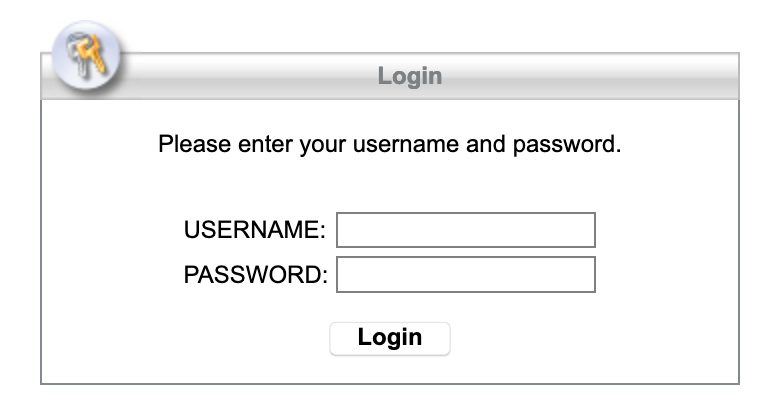
\includegraphics{images/login.png}
\item
  Enter your Purdue Career Account credentials (\textbf{with} BoilerKey).
\item
  Download and install the Cisco AnyConnect Secure Mobility Client.
\item
  Open the AnyConnect client and enter the domain for Purdue's vpn: \texttt{webvpn.purdue.edu}, and click ``Connect'':
  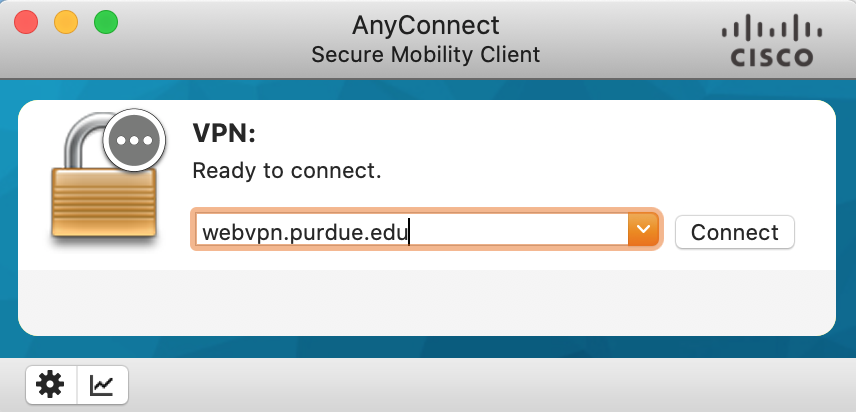
\includegraphics{images/anyconnect.png}
\item
  When prompted, enter your Purdue Career Account credentials (\textbf{with} BoilerKey).
\item
  You should be successfully connected to Purdue's VPN! You can read more about VPNs \protect\hyperlink{vpns}{here}.
\item
  Navigate to \url{https://www.cendio.com/thinlinc/download}, and download the ThinLinc client application for your operating system.
\item
  Install and launch the ThinLinc client:
  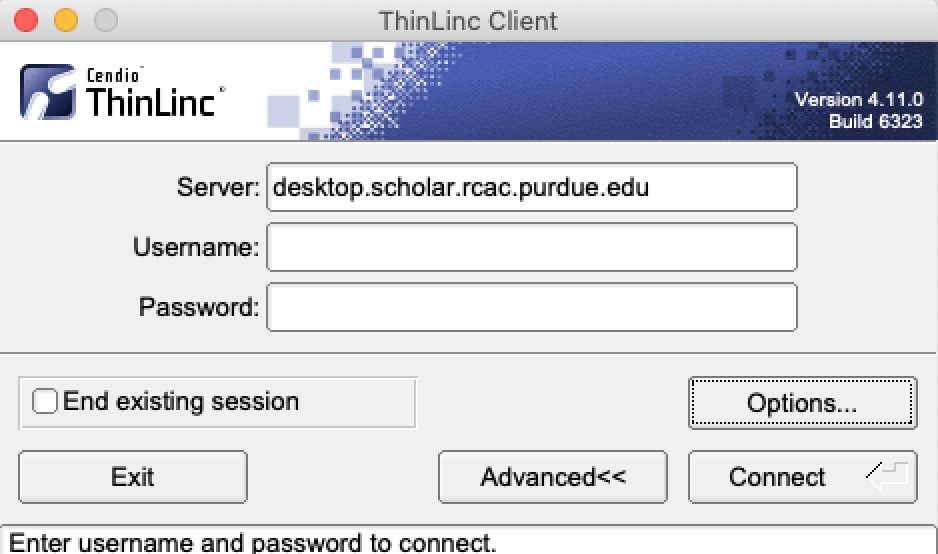
\includegraphics{images/thinlincclient.png}
\item
  Enter your Purdue Career Account information (\textbf{without} BoilerKey), as well as the server: \texttt{desktop.scholar.rcac.purdue.edu}.
\item
  Click on ``Options\ldots{}'' and fill out the ``Screen'' tab as shown below:
  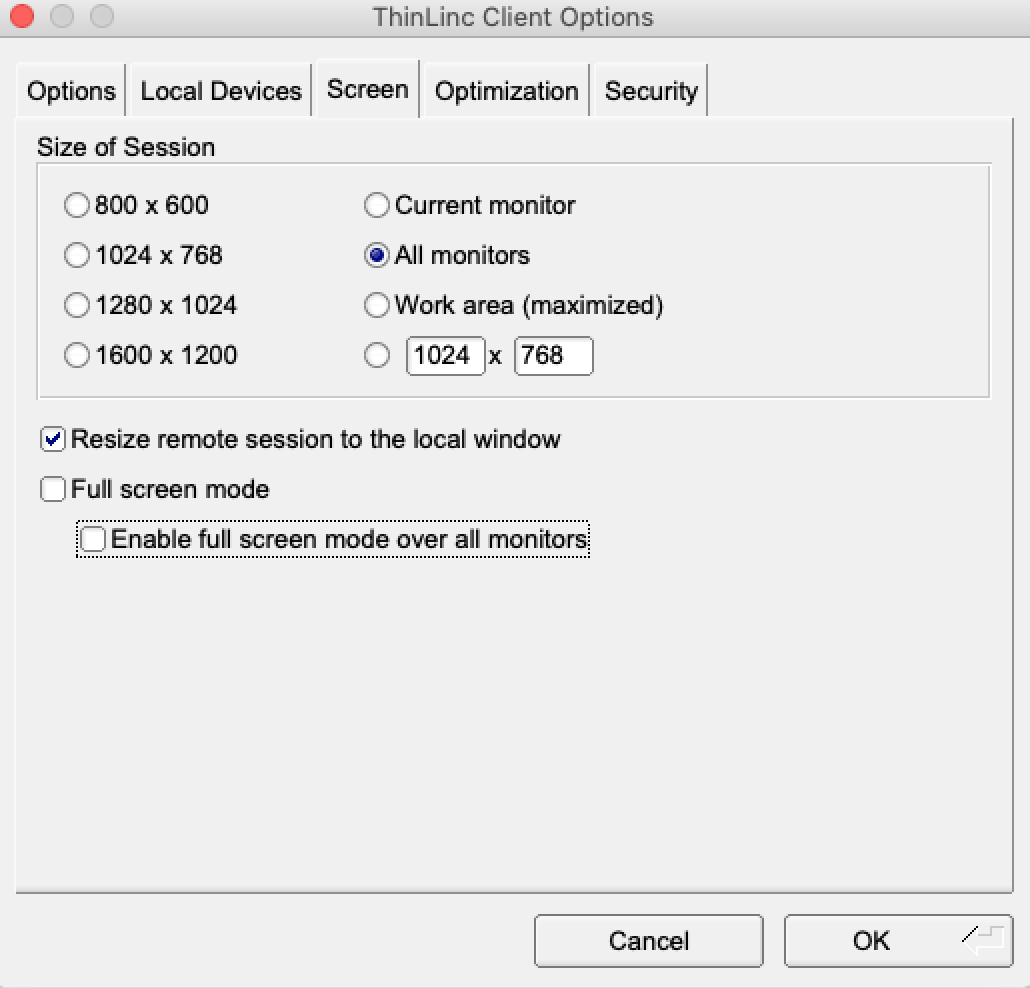
\includegraphics{images/thinlincoptions.png}
\item
  Click ``OK'' and then ``Connect''. \textbf{Make sure you are connected to Purdue's VPN using AnyConnect before clicking ``Connect''!}
\item
  If you are presented with a choice like below, click ``Continue''.
  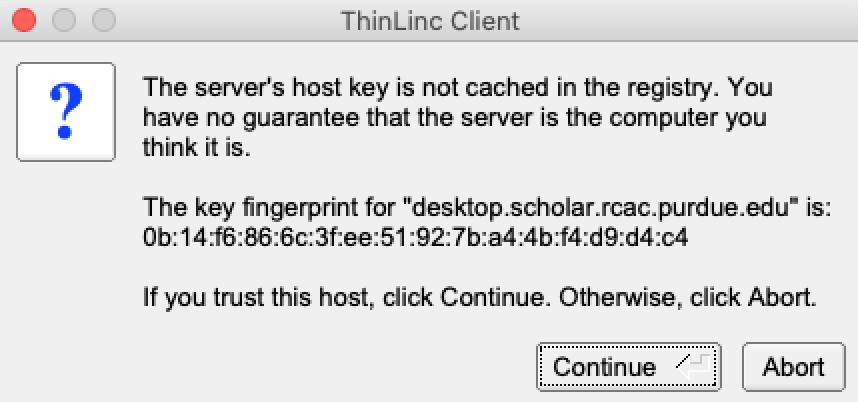
\includegraphics{images/thinlincquestion.png}
\item
  Congratulations, you are now successfully connected to Scholar using the ThinLinc client.
  \textbf{NOTE: If you do accidentally get stuck in full screen mode, the F8 key will help you to escape.}
  \textbf{NOTE: The very first time that you log onto Scholar, you will have an option of ``use default config'' or ``one empty panel''. PLEASE choose the ``use default config''.}
\end{enumerate}

\hypertarget{connecting-with-ssh}{%
\subsection{SSH}\label{connecting-with-ssh}}

\hypertarget{connecting-to-scholar-ssh-windows}{%
\subsubsection{Windows}\label{connecting-to-scholar-ssh-windows}}

\hypertarget{connecting-to-scholar-ssh-macos}{%
\subsubsection{MacOS}\label{connecting-to-scholar-ssh-macos}}

\hypertarget{connecting-to-scholar-ssh-linux}{%
\subsubsection{Linux}\label{connecting-to-scholar-ssh-linux}}

\hypertarget{jupyterhub}{%
\subsection{JupyterHub}\label{jupyterhub}}

\begin{enumerate}
\def\labelenumi{\arabic{enumi}.}
\tightlist
\item
  Open a browser and navigate to \url{https://notebook.scholar.rcac.purdue.edu/}.
\item
  Enter your Purdue Career Account credentials (\textbf{without} BoilerKey).
\item
  Congratulations, you should now be able to create and run Jupyter notebooks on Scholar!
\end{enumerate}

\hypertarget{rstudio-server}{%
\subsection{RStudio Server}\label{rstudio-server}}

\begin{enumerate}
\def\labelenumi{\arabic{enumi}.}
\tightlist
\item
  Open a browser and navigate to \url{https://rstudio.scholar.rcac.purdue.edu/}.
\item
  Enter your Purdue Career Account credentials (\textbf{without} BoilerKey).
\item
  Congratulations, you should now be able to create and run R scripts on Scholar!
\end{enumerate}

\hypertarget{scholar-resources}{%
\section{Resources}\label{scholar-resources}}

\hypertarget{unix}{%
\chapter{Unix}\label{unix}}

\hypertarget{unix-getting-started}{%
\section{Getting started}\label{unix-getting-started}}

\hypertarget{unix-utilities}{%
\section{Standard utilities}\label{unix-utilities}}

\hypertarget{man}{%
\subsection{\texorpdfstring{\texttt{man}}{man}}\label{man}}

\hypertarget{tldr}{%
\subsubsection{\texorpdfstring{\texttt{tldr}}{tldr}}\label{tldr}}

\hypertarget{dots}{%
\subsection{\textasciitilde{} \& . \& ..}\label{dots}}

\hypertarget{cat}{%
\subsection{\texorpdfstring{\texttt{cat}}{cat}}\label{cat}}

\hypertarget{ls}{%
\subsection{\texorpdfstring{\texttt{ls}}{ls}}\label{ls}}

\hypertarget{cp}{%
\subsection{\texorpdfstring{\texttt{cp}}{cp}}\label{cp}}

\hypertarget{mv}{%
\subsection{\texorpdfstring{\texttt{mv}}{mv}}\label{mv}}

\hypertarget{pwd}{%
\subsection{\texorpdfstring{\texttt{pwd}}{pwd}}\label{pwd}}

\hypertarget{touch}{%
\subsection{\texorpdfstring{\texttt{touch}}{touch}}\label{touch}}

\hypertarget{wc}{%
\subsection{\texorpdfstring{\texttt{wc}}{wc}}\label{wc}}

\hypertarget{ssh}{%
\subsection{\texorpdfstring{\texttt{ssh}}{ssh}}\label{ssh}}

\hypertarget{mosh}{%
\subsubsection{\texorpdfstring{\texttt{mosh}}{mosh}}\label{mosh}}

\hypertarget{scp}{%
\subsection{\texorpdfstring{\texttt{scp}}{scp}}\label{scp}}

\hypertarget{awk}{%
\subsection{\texorpdfstring{\texttt{awk}}{awk}}\label{awk}}

\hypertarget{sed}{%
\subsection{\texorpdfstring{\texttt{sed}}{sed}}\label{sed}}

\hypertarget{grep}{%
\subsection{\texorpdfstring{\texttt{grep}}{grep}}\label{grep}}

\hypertarget{rg}{%
\subsubsection{\texorpdfstring{\texttt{ripgrep}}{ripgrep}}\label{rg}}

\hypertarget{find}{%
\subsection{\texorpdfstring{\texttt{find}}{find}}\label{find}}

\hypertarget{fd}{%
\subsubsection{\texorpdfstring{\texttt{fd}}{fd}}\label{fd}}

\hypertarget{top}{%
\subsection{\texorpdfstring{\texttt{top}}{top}}\label{top}}

\hypertarget{less-and-more}{%
\subsection{\texorpdfstring{\texttt{less} \& \texttt{more}}{less \& more}}\label{less-and-more}}

\hypertarget{sort}{%
\subsection{\texorpdfstring{\texttt{sort}}{sort}}\label{sort}}

\hypertarget{piping-and-redirection}{%
\section{Piping \& Redirection}\label{piping-and-redirection}}

\hypertarget{emacs}{%
\section{Emacs}\label{emacs}}

\hypertarget{nano}{%
\section{Nano}\label{nano}}

\hypertarget{vim}{%
\section{Vim}\label{vim}}

\hypertarget{writing-scripts}{%
\section{Writing scripts}\label{writing-scripts}}

\hypertarget{sql}{%
\chapter{SQL}\label{sql}}

\hypertarget{rdbms}{%
\subsection{RDBMS}\label{rdbms}}

\hypertarget{sql-in-r}{%
\subsection{SQL in R}\label{sql-in-r}}

\hypertarget{sql-in-python}{%
\subsection{SQL in Python}\label{sql-in-python}}

\hypertarget{r}{%
\chapter{R}\label{r}}

\hypertarget{getting-started-with-r}{%
\section{Getting started}\label{getting-started-with-r}}

How to install R (windows/mac/linux)
How to install RStudio
How to connect to RStudio Server on Scholar
How to get help (?, help(), get function itself)

\hypertarget{r-variables}{%
\section{Variables}\label{r-variables}}

\hypertarget{r-logical-operators}{%
\section{Logical operators}\label{r-logical-operators}}

\hypertarget{r-lists-and-vectors}{%
\section{Lists \& Vectors}\label{r-lists-and-vectors}}

\hypertarget{r-basic-functions}{%
\section{Basic R functions}\label{r-basic-functions}}

\hypertarget{r-data-frames}{%
\section{Data.frames}\label{r-data-frames}}

\hypertarget{r-reading-and-writing-data}{%
\section{Reading \& Writing data}\label{r-reading-and-writing-data}}

\hypertarget{r-control-flow}{%
\section{Control flow}\label{r-control-flow}}

\hypertarget{r-apply-functions}{%
\section{Apply functions}\label{r-apply-functions}}

\hypertarget{r-apply}{%
\subsection{\texorpdfstring{\texttt{apply}}{apply}}\label{r-apply}}

\hypertarget{r-sapply}{%
\subsection{\texorpdfstring{\texttt{sapply}}{sapply}}\label{r-sapply}}

\hypertarget{r-lapply}{%
\subsection{\texorpdfstring{\texttt{lapply}}{lapply}}\label{r-lapply}}

\hypertarget{r-tapply}{%
\subsection{\texorpdfstring{\texttt{tapply}}{tapply}}\label{r-tapply}}

\hypertarget{r-writing-functions}{%
\section{Writing functions}\label{r-writing-functions}}

\hypertarget{r-plotting}{%
\section{Plotting}\label{r-plotting}}

\hypertarget{r-ggplot2}{%
\subsection{\texorpdfstring{\texttt{ggplot2}}{ggplot2}}\label{r-ggplot2}}

\hypertarget{r-rmarkdown}{%
\section{RMarkdown}\label{r-rmarkdown}}

\hypertarget{r-tidyverse}{%
\section{Tidyverse}\label{r-tidyverse}}

\hypertarget{r-datatable}{%
\section{data.table}\label{r-datatable}}

\hypertarget{r-sql}{%
\section{SQL in R}\label{r-sql}}

\hypertarget{r-scraping}{%
\section{Scraping}\label{r-scraping}}

\hypertarget{r-shiny}{%
\section{\texorpdfstring{\texttt{shiny}}{shiny}}\label{r-shiny}}

\hypertarget{python}{%
\chapter{Python}\label{python}}

\hypertarget{getting-started-with-python}{%
\section{Getting started}\label{getting-started-with-python}}

\hypertarget{p-lists-and-tuples}{%
\section{Lists \& Tuples}\label{p-lists-and-tuples}}

\hypertarget{p-dicts}{%
\section{Dicts}\label{p-dicts}}

\hypertarget{p-control-flow}{%
\section{Control flow}\label{p-control-flow}}

\hypertarget{p-writing-functions}{%
\section{Writing functions}\label{p-writing-functions}}

\hypertarget{p-reading-and-writing-data}{%
\section{Reading \& Writing data}\label{p-reading-and-writing-data}}

\hypertarget{p-numpy}{%
\section{\texorpdfstring{\texttt{numpy}}{numpy}}\label{p-numpy}}

\hypertarget{p-scipy}{%
\section{\texorpdfstring{\texttt{scipy}}{scipy}}\label{p-scipy}}

\hypertarget{p-pandas}{%
\section{\texorpdfstring{\texttt{pandas}}{pandas}}\label{p-pandas}}

\hypertarget{p-jupyter-notebooks}{%
\section{Jupyter notebooks}\label{p-jupyter-notebooks}}

\hypertarget{p-writing-scripts}{%
\section{Writing scripts}\label{p-writing-scripts}}

\hypertarget{p-argparse}{%
\subsection{\texorpdfstring{\texttt{argparse}}{argparse}}\label{p-argparse}}

\hypertarget{p-scraping}{%
\section{Scraping}\label{p-scraping}}

\hypertarget{p-plotting}{%
\section{Plotting}\label{p-plotting}}

\hypertarget{p-matplotlib}{%
\subsection{\texorpdfstring{\texttt{matplotlib}}{matplotlib}}\label{p-matplotlib}}

\hypertarget{p-plotly}{%
\subsection{\texorpdfstring{\texttt{plotly}}{plotly}}\label{p-plotly}}

\hypertarget{p-plotnine}{%
\subsection{\texorpdfstring{\texttt{plotnine}}{plotnine}}\label{p-plotnine}}

\hypertarget{p-pygal}{%
\subsection{\texorpdfstring{\texttt{pygal}}{pygal}}\label{p-pygal}}

\hypertarget{p-seaborn}{%
\subsection{\texorpdfstring{\texttt{seaborn}}{seaborn}}\label{p-seaborn}}

\hypertarget{p-bokeh}{%
\subsection{\texorpdfstring{\texttt{bokeh}}{bokeh}}\label{p-bokeh}}

\hypertarget{p-classes}{%
\section{Classes}\label{p-classes}}

\hypertarget{tensorflow}{%
\section{\texorpdfstring{\texttt{tensorflow}}{tensorflow}}\label{tensorflow}}

\hypertarget{pytorch}{%
\section{\texorpdfstring{\texttt{pytorch}}{pytorch}}\label{pytorch}}

\hypertarget{tools}{%
\chapter{Tools}\label{tools}}

\hypertarget{docker}{%
\section{Docker}\label{docker}}

\hypertarget{tableau}{%
\section{Tableau}\label{tableau}}

\hypertarget{github}{%
\section{GitHub}\label{github}}

\hypertarget{vpns}{%
\section{VPNs}\label{vpns}}

\hypertarget{faqs}{%
\chapter{FAQs}\label{faqs}}

\hypertarget{how-do-i-connect-to-scholar-from-off-campus}{%
\section{How do I connect to Scholar from off-campus?}\label{how-do-i-connect-to-scholar-from-off-campus}}

There are a variety of ways to connect to Scholar from off-campus. You can \protect\hyperlink{connecting-with-thinlinc-webclient}{use the ThinLinc web client}, or \protect\hyperlink{connecting-with-thinlinc-client}{setup a VPN connection to Purdue's VPN, and connect using the ThinLinc client application}. If you just want to use Jupyter notebooks, you can \protect\hyperlink{jupyterhub}{use JupyterHub}. If you just want to use RStudio, you can \protect\hyperlink{rstudio-server}{use RStudio Server}.

\hypertarget{is-there-an-advantage-to-using-the-thinlinc-client-rather-than-the-thinlinc-web-client}{%
\section{Is there an advantage to using the ThinLinc client rather than the ThinLinc web client?}\label{is-there-an-advantage-to-using-the-thinlinc-client-rather-than-the-thinlinc-web-client}}

Yes. Although it is marginally more difficult to connect with, the ThinLinc client allows the user to copy and paste directly from their native operating system. So for example, if you have an RStudio session opened on your MacBook, you can directly copy and paste code onto Scholar using the ThinLinc client. You are unable to do this via the ThinLinc web client.

\hypertarget{github-classroom-is-not-working-cant-authorize-the-account.}{%
\section{GitHub Classroom is not working -- can't authorize the account.}\label{github-classroom-is-not-working-cant-authorize-the-account.}}

This is usually a browser issue. GitHub Classroom does not work well with Microsoft Edge or Internet Explorer. Try \href{https://www.mozilla.org/en-US/firefox/new/}{Firefox} or Safari or \href{https://www.google.com/chrome/}{Chrome}.

\hypertarget{in-scholar-my-font-size-looks-weird-or-my-cursor-is-offset.}{%
\section{In Scholar, my font size looks weird or my cursor is offset.}\label{in-scholar-my-font-size-looks-weird-or-my-cursor-is-offset.}}

In scholar, navigate to \texttt{Tools\ \textgreater{}\ Global\ Options\ \textgreater{}\ Appearance}, and select the ``Monospace'' font, and click the ``Apply'' button.

\hypertarget{how-do-i-make-the-thinlinc-window-bigger-without-going-to-the-dreaded-full-screen-mode}{%
\section{How do I make the ThinLinc window bigger without going to the dreaded ``full screen'' mode?}\label{how-do-i-make-the-thinlinc-window-bigger-without-going-to-the-dreaded-full-screen-mode}}

See \href{https://home.cc.umanitoba.ca/~psgendb/local/public_html/remote/desktop/thinlinc/thinlinc.local.html}{here}.

\hypertarget{im-unable-to-type-into-the-terminal-in-rstudio.}{%
\section{I'm unable to type into the terminal in RStudio.}\label{im-unable-to-type-into-the-terminal-in-rstudio.}}

Try opening a new terminal, try clearing the terminal buffer, or interrupting the current terminal. All these options come from a menu that will pop up when you hit the small down arrow next to the words ``Terminal 1'' (it might be another number depending on how many terminals are open) which is on the left side right above the terminal in RStudio.~

\hypertarget{im-unable-to-connect-to-rstudio-server.}{%
\section{I'm unable to connect to RStudio Server.}\label{im-unable-to-connect-to-rstudio-server.}}

Try closing it, clearing your cookies, and using the original link: \url{https://rstudio.scholar.racac.purdue.edu/}, or for ease of scrolling, try \url{https://desktop.scholar.rcac.purdue.edu}, and open up RStudio from within the ThinLinc web client.

\hypertarget{section}{%
\section{}\label{section}}

\hypertarget{contributors}{%
\chapter{Contributors}\label{contributors}}

We are extremely thankful for all of our contributors! Get your name added to the list by \protect\hyperlink{how-to-contribute}{making a contribution}.

\end{document}
